\documentclass[11pt]{scrartcl}

% French
\usepackage[utf8]{inputenc}
\usepackage[T1]{fontenc}
\usepackage[frenchb]{babel}

\usepackage{hyperref}
\hypersetup{
    colorlinks,
    linkcolor={red!50!black},
    citecolor={blue!50!black},
    urlcolor={blue!30!black}
}

\usepackage{dirtree}
\usepackage{graphicx}
\graphicspath{{images/}}

% Specifying the outputdir option else a bug prevents from compiling a document that contains in-doc minted code.
\usepackage[outputdir=/tmp]{minted}

\usepackage[usenames,dvipsnames]{xcolor}

\definecolor{darkblue}{HTML}{123C73}
\definecolor{darkbrown}{HTML}{A16516}

\newcommand{\funname}[1]{\texttt{\textcolor{darkblue}{#1}}}
\newcommand{\filename}[1]{\texttt{\textcolor{darkbrown}{#1}}}
\newcommand{\code}[1]{\mintinline{ocaml}{#1}}

%% This code substitutes underscore.sty
\begingroup\lccode`~=`_
\lowercase{\endgroup
  \protected\def~{\ifmmode\sb\else\textunderscore\fi}
}
\AtBeginDocument{\catcode`_=\active}
%% end

\usepackage{fancyhdr}
\pagestyle{fancy}
\fancyhf{}
\fancyhead[LE,RO]{Quentin Barrand}
\fancyhead[RE,LO]{ENSIIE \\ IPRF - « QuadTree »}
\fancyfoot[LE,CO]{\thepage}

 \areaset[5mm]{412pt}{657pt}

\begin{document}

\title{\textbf{IPRF - « QuadTree »}}
\subtitle{Rapport}

\author{Quentin Barrand\\
		\href{mailto:quentin@quba.fr}{\texttt{quentin@quba.fr}}}
		
\date{\today}

\maketitle

\begin{abstract}
Ce document a été réalisé dans le cadre du projet final du module IPRF \mbox{« Programmation fonctionnelle »} de la formation FIPA de l'ENSIIE.\\
Dans ce projet, nous étudions l'opportunité d'utiliser une structure de données de type arbre 4-aire (« QuadTree ») pour stocker des points appartenant à un repère orthonormé; le but de détecter des collisions entre un disque en déplacement et des obstacles matérialisés par ces points.\\
Le QuadTree étudié dans ce projet n'est pas extensible (les bornes du plan donné à l'initialisation sont fixes et positives) et possède une taille de panier égale à 1, ce qui signifie qu'un seul objet peut être stocké par nœud terminal.\\
Ce projet est l'occasion d'étudier plusieurs stratégies de stockage d'objets en mémoire et d'approfondir l'utilisation de la bibliothèque standard d'OCaml pour des usages graphiques.
\end{abstract}

\break

\section*{Organisation du projet}
Pour chaque section, les fonctions à écrire sont dans les fichiers \filename{partX.ml} et le code interactif (tel que les tests graphiques) dans les fichiers \filename{partX.test.ml}. Cette organisation permet d'importer le code des sections précédentes à l'aide de directives \mintinline{ocaml}{#use} sans provoquer des appels de fonction inattendus.
\\
Le rendu est donc constitué des fichiers suivants :
\dirtree{%
 .1 /.
 .2 bonus.ml\DTcomment{Bonus}.
 .2 coord.ml\DTcomment{Partie 1}.
 .2 display.ml\DTcomment{Fourni par le sujet}.
 .2 part1.test.ml\DTcomment{Partie 1 - tests}.
 .2 part2.test.ml\DTcomment{Partie 2 - tests}.
 .2 part3.ml\DTcomment{Partie 3}.
 .2 part3.test.ml\DTcomment{Partie 3 - tests}.
 .2 part4.ml\DTcomment{Partie 4}.
 .2 part4.test.ml\DTcomment{Partie 4 - tests}.
 .2 part5.ml\DTcomment{Partie 5}.
 .2 part5.test.ml\DTcomment{Partie 5 - tests}.
 .2 quadtree.ml\DTcomment{Partie 2}.
 .2 rect.ml\DTcomment{Partie 1}.
 .2 report.pdf\DTcomment{Le présent rapport au format PDF}.
 .2 report.tex\DTcomment{Le présent rapport au format \LaTeX}.
 .2 simulation1.ml\DTcomment{Fourni par le sujet}.
 .2 simulation2.ml\DTcomment{Fourni par le sujet}.
}


\section{Échauffement sur les rectangles}

\begin{description}
\item[Question 1.] Voir \filename{rect.ml}.

\item[Question 2.] Voir \filename{rect.ml}.

\item[Question 3.] Voir \filename{rect.ml}.

\item[Question 4.] Voir \filename{rect.ml}.

\item[Question 5.] Voir \filename{rect.ml}.

\item[Question 6.] Voir \filename{rect.ml}.
\end{description}

\section{La structure de données QuadTree}

\begin{description}
\item[Question 7.] Pour stocker une collection de points, on pourrait utiliser quatre grandes familles de structures de données :
\begin{description}
\item[Ensembles ou listes] On stocke les coordonnées des points les uns à la suite des autres dans une liste.\\
Occupation mémoire : minimale ($n \times taille(n)$).\\
Algorithmes d'accès : très peu efficaces (parcours de la liste - $\mathcal{O}(n)$).
\item[Dictionnaires] On stocke les points dans un dictionnaire dont les clés sont les coordonnées des points.\\
Occupation mémoire : Modérée (on considère que pour éviter la plupart des collisions sur la fonction de hachage, il est nécessaire de d'utiliser un ensemble environ 5 fois plus grand que le nombre d'éléments à stocker -- $5 \times n \times taille(n)$).\\
Algorithmes d'accès : très efficaces lorsque l'on connaît les coordonnées exactes du point (temps quasi-constant qui dépend de la fonction de hachage choisie et du nombre d'éléments possédant la même clé), peu efficaces dans les autres cas (recherche de tous les points contenus dans une restriction du plan initial par exemple) puisqu'il est nécessaire de parcourir tout le dictionnaire ($\mathcal{O}(n)$).
\item[Matrices] On stocke un tableau à deux dimensions en mémoire, et aux coordonnées du point dans la matrice on stocke l'objet lié au point.\\
%Toutefois, cette structure de données peut se révéler inadaptée aux stockage de points aux coordonnées représentées par des nombres flottants, en raison de la façon dont ils sont représentés en mémoire.\\
Occupation mémoire : très importante (de l'ordre de $((Abs_{max} - Abs_{min}) \times (Ord_{max} - Ord_{min})) \times taille(n)$).\\
Algorithmes d'accès : très efficaces (temps quasi-constant qui dépend seulement du nombre d'éléments possédant la même clé).
\item[Arbres n-aires] Les arbres permettent de combiner une utilisation mémoire modérée et une recherche efficace. L'emploi du QuadTree, arbre 4-aire, est particulèrement justifié pour travailler avec des points 2D, puisqu'il découpe si nécessaire le plan en rectangles successifs et que tout point est logiquement contenu dans un rectangle. Ainsi, la recherche de tous les points contenus dans une restriction du plan initial est très rapide.\\
Occupation mémoire : modérée ($\leq 4 \times n \times taille(n)$).\\
Algorithmes d'accès : efficaces ($\mathcal{O}(\log{}n)$).
\end{description}
\item[Question 8.] Voir \filename{quadtree.ml}.

\item[Question 9.] Voir \filename{quadtree.ml}.

\item[Question 10.] Voir \filename{quadtree.ml}.

\item[Question 11.] Voir \filename{quadtree.ml}.

\item[Question 12.] Voir \filename{quadtree.ml}.

\item[Question 13.] Voir \filename{quadtree.ml}.\\
Intuitivement, on pourrait être tenté d'utiliser \funname{list_of_quadtree}, puis de supprimer l'élément choisi dans la liste, puis de faire de nouveau appel à \funname{quadtree_of_list}; la fonction \funname{list_remove} implémente cette méthode.\\
Pour éviter l'opération en $\mathcal{O}(n)$ qui consiste à reconstruire le QuadTree après avoir supprimé un objet dans la liste, on peut écrire une fonction \funname{clean_qt} qui devrait permettre d'avoir une simplification plus performante du QuadTree que si l'on utilisait la méthode décrite plus haut. Malgré de nombreux tests, nous n'avons pas trouvé de cas dans lesquels cette fonction produirait des résultats incorrects.
\end{description}

\section{Représentation graphique d'un QuadTree et tests}

\begin{description}
\item[Question 14.] Fonctions de \filename{display.ml} :
\begin{description}
\item[\funname{draw_data}] Dessine une donnée stockée dans une feuille \code{Leaf of coord * 'a} d'un QuadTree. La fonction de conversion de \code{'a} vers \code{String} ainsi que la couleur de dessin doivent être passées en paramètres.
\item[\funname{draw_quadtree}] Dessine récursivement un QuadTree. Commence par dessiner en bleu le rectangle dans lequel est contenu le QuadTree, puis, en fonction de la nature de l'élement \code{cell} :
\begin{itemize}
\item ne fait rien si l'élément est \code{Empty};
\item fait appel à \funname{draw_data} si l'élément est \code{Leaf};
\item s'appelle récursivement pour chaque sous-QuadTree si l'élément est \code{Node}.
\end{itemize}
\item[\funname{wait_and_quit}] Attend un appui sur une touche du clavier puis ferme la fenêtre de dessin.
\item[\funname{init}] Initialise un environnement de dessin en fonction de la taille du rectangle passé en paramètre et ouvre la fenêtre. Retourne un triplet de \code{Float} nommé \code{dparams} dans le reste du projet et utilisé par toutes les fonctions de dessin. 
\item[\funname{simple_test}] Appelle la fonction \funname{draw_quadtree} à l'aide du triplet \code{dparams} (obtenu par un précédent appel à la fonction \funname{init}) et d'une fonction de conversion vers le type \code{String} pour dessiner le QuadTree passé en paramètre.
\end{description}

\item[Question 15.] Voir \filename{part3.ml}.\\
La fonction \funname{new_simple_test} prend en paramètre deux coordonnées \code{c} et \code{c'} et un entier \code{n}. Elle insère dans un QuadTree vide délimité par le rectangle formé par \code{c} et \code{c'} \code{n} objets dont les coordonnées sont obtenues aléatoirement à l'aide du module \code{Random}. Elle affiche le QuadTree ainsi complété, puis lors de l'appui sur une touche, le vide et l'affiche de nouveau. De cette façon, on peut vérifier que tous les objets sont bien supprimés.\\
Un appel à cette fonction avec l'insertion d'une centaine d'objets est disponible dans le fichier \filename{part3.test.ml}.

\item[Question 16.] Voir \filename{part3.ml}.\\
En utilisant \code{rect_length} et \code{rect_height}, dans la fonction \funname{bad_draw_quadtree}, on observe que certains segments délimitant les bordures du QuadTrees sont plus épais que d'autres (voir Fig.~\ref{q16goodquadtree} et \ref{q16badquadtree}). Le problème peut être lié à plusieurs conversions de nombres flottants en entiers :
\begin{itemize}
	\item Lorsque l'on utilise la fonction \funname{draw_quadtree}, la conversion de nombre flottant en nombre entier a lieu une fois que le calcul sur les composantes flottantes \code{sx} / \code{sy}, \code{rect_left r} / \code{rect_right r} / \code{rect_top r} / \code{rect_bottom r} et \code{z} est terminé; on a donc un seul arrondi.
	\item Lorsque l'on utilise la fonction \funname{bad_draw_quadtree}, on additionne le résultat arrondi en entier du calcul sur les deux composantes flottantes \code{z} et \code{rect_length r} / \code{rect_height r} à la composante entière déjà arrondie \code{x1} ou \code{x2}; on fait alors deux arrondis, qui peuvent provoquer le dessin de traits non superposés lorsque l'on dessine plusieurs fois le même QuadTree.
Ces traits proches mais non superposés
apparaissent dans la fenêtre graphique comme des traits plus épais.
\end{itemize}

\begin{figure}[!h]
	\centering
	\fbox{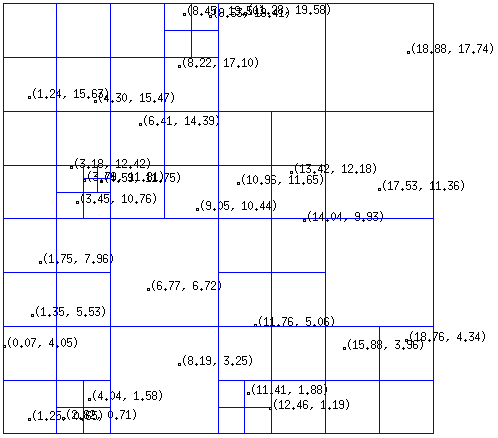
\includegraphics[scale=0.6]{q16goodquadtree.png}}
	\caption{\label{q16goodquadtree} Un exemple de dessin d'un QuadTree \code{q} en utilisant la fonction \funname{simple_test} fournie par le sujet.}
\end{figure}

\begin{figure}[!h]
	\centering
	\fbox{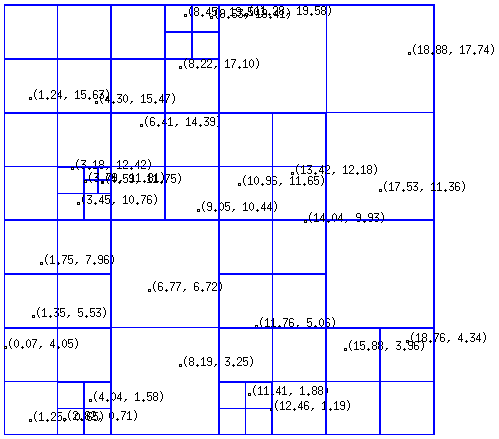
\includegraphics[scale=0.6]{q16badquadtree.png}}
	\caption{\label{q16badquadtree} Un exemple de dessin du même QuadTree \code{q} que dans la Fig.~\ref{q16goodquadtree}, en utilisant cette fois la fonction buggée \funname{bad_simple_test}.}
\end{figure}

\clearpage

\end{description}

\section{Placement du disque}

\begin{description}
\item[Question 17.] Voir \filename{part4.ml}.

\item[Question 18.] Voir \filename{part4.ml}.

\item[Question 19.] Voir \filename{part4.ml}.

\item[Question 20.] Fonctions de \filename{simulation1.ml} :
\begin{description}
\item[\funname{get_point}] Retourne les coordonnées du point sur lequel se trouve le pointeur de la souris lors du déclenchement du clic.
\item[\funname{get_disk}] Retourne les coordonnées du centre et la longueur du rayon du cercle désigné par une action « clic - glisser » (début du clic - déplacement du pointeur - relâchement du pointeur).
\item[\funname{draw_disk}] Dessine à disque d'une couleur spécifiée à des coordonnées spécifiées, plein ou non.
\item[\funname{draw_disk_with_collisions}] Dessine un disque :
\begin{itemize}
\item de couleur jaune s'il recouvre des points du QuadTree (obtenus grâce à \funname{collision_disk} de \filename{part4.ml}), et fait appel à \funname{draw_data} de \filename{display.ml} pour dessiner ces points en rouge le cas échéant;
\item de couleur verte sinon.
\end{itemize}
\item[\funname{simulation_placement}] Fait appel aux fonctions \funname{init} et \funname{draw_quadtree} de \\ \filename{display.ml} et aux fonctions \funname{get_disk} et \funname{draw_disk_with_collisions} pour dessiner un cercle défini à la souris par l'utilisateur et ses éventuels collisions avec les points du QuadTree.
\end{description}
\end{description}

\section{Déplacement du disque et détection de collision}

\begin{description}
\item[Question 21.] Voir \filename{part5.ml}.

\item[Question 22.] Voir \filename{part5.ml}.

\item[Question 23.] Voir \filename{part5.test.ml}.\\
Fonctions de \filename{simulation2.ml} :
\begin{description}
\item[\funname{draw_trail_with_collisions}] Dessine la zone survolée pendant le cercle pendant son déplacement depuis son point de départ vers son point d'arrivée. Fait appel à \funname{collision_trail} pour obtenir une liste tous les points survolés. Redessine ensuite tous ces points en cyan.
\item[\funname{simulation_move}] Idem que \funname{simulation_placement} de \filename{simulation1.ml}, sauf \\ qu'après avoir défini un cercle, un second clic de souris utilise la fonction \funname{draw_trail_with_collisions} pour déplacer le cercle vers cette seconde position. Un exemple de fonctionnement de cette fonction est disponible plus bas (voir Fig.~\ref{q23}).
\end{description}
Dans \filename{part5.ml}, on trouvera également les fonctions \funname{get_new_destination} et \\ \funname{new_simulation_move} qui implémentent le bonus de la question. Une illustration du fonctionnement de ces fonctions est disponible plus bas (voir Fig.~\ref{q23bonus}).

\begin{figure}[h]
	\centering
	\fbox{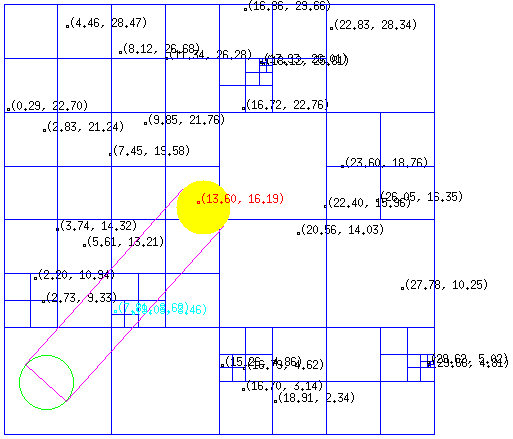
\includegraphics[scale=0.6]{q23.png}}
	\caption{\label{q23} Illustration du fonctionnement de la fonction \funname{simulation_move}.}
\end{figure}

\begin{figure}[h]
	\centering
	\fbox{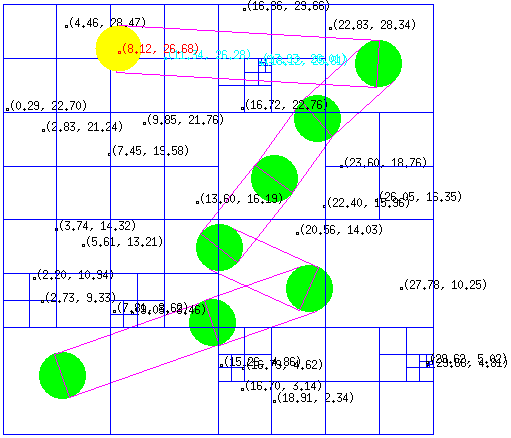
\includegraphics[scale=0.6]{q23bonus.png}}
	\caption{\label{q23bonus} Illustration du fonctionnement de la fonction bonus \funname{new_simulation_move}.}
\end{figure}

\clearpage

\end{description}

\section*{Bonus}
A l'origine écrite pour débugger \funname{clip}, la fonction \funname{graphical_clip} du fichier \filename{bonus.ml} doit permettre de réaliser de façon graphique une restriction du plan, comme suggéré dans la Fig.~2 du sujet. Elle prend en paramètre un QuadTree et une fonction d'affichage des données du QuadTree; cependant, bien qu'elle semble produire un QuadTree correct, il est impossible de l'afficher correctement. 

\section*{Conclusion}
L'arbre 4-aire (« QuadTree ») possède des propriétés très intéressantes pour le stockage de données géographiques dans un plan. D'une part, les algorithmes d'accès à une donnée en particulier sont raisonnablement rapides ($\mathcal{O}(\log{}n)$); d'autre part, l'empreinte mémoire est faible en comparaison avec d'autres structures de données de performance comparable. Les QuadTrees permettent également de restreindre assez facilement l'espace de recherche à une sous-partie du plan initial (voir la fonction \funname{clip} dans la partie 4), et la visualisation de leur contenu pour le débuggage est assez intuitive.
\\
Dans ce projet, nous avons vu un cas d'utilisation typique des QuadTrees : la détection de collisions. Les algorithmes développés plus haut sont couramment utilisés dans le monde des jeux vidéos par exemple puisqu'ils permettent de ne tester la collision de l'objet en mouvement qu'avec une partie des points du plan du plan complet, ce qui réduit considérablement les calculs.
\\
Il est également possible de généraliser cette structure de données pour gérer des objets en trois dimensions dans l'espace, en utilisant des arbres 8-aires (« OctTrees »).


\end{document}
